\section{Computational methods}
\label{chap1:sec:computational_methods}

In the multidisciplinary field of the computational modelling, the development of accurate and efficient numerical methods has been a topic of extensive research.
In that regard, uncountable spatial discretization methods have emerged, where three commonly used classes of methods are relevant to mention, namely the finite difference method, the finite element method, and the finite volume method.
Notice that time discretization methods for unsteady mathematical models are not in the scope of the present work.
In any case, as described in Section~\ref{chap1:sec:computational_modelling}, the general strategy consists in transforming the partial differential equations into a system of algebraic equations, each relating a set of local mesh variables, which is then solved with matrix algebra techniques.
These methods are briefly described hereafter, where a particular focus is given to the finite volume method, which is the approach employed in the present work.

\subsection{Discretization methods}
\label{chap1:subsec:computational_methods_discretization_methods}

The finite difference method is one of the simplest and oldest discretization technique, which has been historically used in the context of computational fluid dynamics problems~\cite{chap1:1998tveito,chap1:1998thomas,chap1:2007grossmann}.
The discretization technique in the finite difference method is based on a truncated Taylor series expansion to approximate the derivatives in the partial differential equations in each cell of the mesh.
A derivative of a specific order, in a truncated Taylor series, is approximated as a difference between the derivatives of previous order at the cell points, divided by the distance between the cell points.
Similarly, the derivatives in the partial differential equations are approximated in terms of discrete variables in the vicinity of each cell.
Then, all the equations are assembled in a system of linear equations, which is solved with matrix algebra techniques.
Although the derivation of the finite difference method is straightforward, only orthogonal structured grids are handled since the alignment of the cell points in each direction is required to derive the appropriate finite differences.

The finite element method is another popular discretization technique, which has been predominantly used in structural problems for the analysis of stress and deformation in solids~\cite{chap1:1993reddy,chap1:2004ern,chap1:2005chen,chap1:2005zienkiewicza,chap1:2005zienkiewiczb}.
The discretization technique in the finite element method is based on a variational formulation of the partial differential equation with an error functional to minimize, which provides an approximation of the physical variables, as proved from the calculus of variations.
The finite element method requires basis or shape functions defined for reference elements (such as triangles and quadrilaterals), which are then mapped onto the cells.
Although the discrete variables are always defined at the vertices, the choice of basis functions provides several derivations of the finite element method.
Contrarily to the classical finite difference method, the finite element method does not require a fixed simple mesh structure and, therefore, is capable of handling complex geometries with relative ease, when compared with the former.
The linear algebraic equations derived from the method are then assembled in a system of linear equations, which is solved with matrix algebra techniques.
However, the derivation of the finite element method requires significant knowledge of calculus of variations and, therefore, is conceptually more complicated than the finite difference method.

The finite volume method is one of the most classical discretization techniques in computational fluid dynamics and has been receiving significant attention since the eighties with the pioneering work of Patankar on heat transfer and fluid flow problems~\cite{chap1:1980patankar}.
In comparison with the finite difference method and the finite element method, the extensive use of the finite volume method is recent, although its foundations date back to the early 1970s, previously to the work of Patankar.
Posteriorly, the method seems to had been independently used to compute approximations of hyperbolic conservation law systems of compressible gas dynamics in the works of P.W. McDonald, 1971~\cite{chap1:1971mcdonald}, in the American Society of Mechanical Engineers (ASME) and of R.W. MacCormack et al., 1972~\cite{chap1:1972maccormack}, and A.W. Rizzi et al., 1973~\cite{chap1:1973rizzi}, in the American Institute of Aeronautics and Astronautics (AIAA).
Moreover, the seminal works of B.V. Leer, 1973--1979~\cite{chap1:1973leer,chap1:1974leer,chap1:1976leer,chap1:1977leera,chap1:1977leerb,chap1:1979leer}, and the works of V.P. Kolgan, 1972--1975~\cite{chap1:1972kolgan,chap1:1975kolgana,chap1:1975kolganb}, were also remarkable in the early development of the finite volume method for hyperbolic conservation problems.
However, some authors claim that the main ideas and principles of the finite volume method are even older and date back to the early 1960s.
For instance, the work of S.K. Godunov, 1959~\cite{chap1:1959godunov}, and A. Preissmann, 1961~\cite{chap1:1961preissmann}, advocating a box scheme to solve the Saint-Venant equations in hydraulic flow problems, can be regarded as one of the basic finite volume formulations.
Additionally, the work of R.S. Varga, 1962~\cite{chap1:1962varga}, to solve self-adjoint elliptic equations using an integration approach to derive finite difference approximations was standard practice in nuclear research at that time.
The works conducted by A.N. Tichnov et al., 1962~\cite{chap1:1962tichonov}, and by A.A. Samarskii, 1965~\cite{chap1:1965samarskii}, can also be considered as precursors of the finite volume method, although the historical background from the USSR side is scarce.
Nevertheless, the method did not receive much attention during those three decades while the finite element method was seeing a noticeable expansion for the physicists and engineers.

\subsection{Finite volume method}
\label{chap1:subsec:computational_methods_finite_volume_method}

The finite volume method is applied to the integral form of the partial differential equations, usually having a divergence term of some physical variable.
The divergence or Gauss's theorem is fundamental in the finite volume method, allowing to convert the volume integral over some finite control volume into a surface integral.
For instance, consider some control volume denoted as $V$, with surface denoted as $S$, and unit normal vector denoted as $\bm{n}$, as illustrated in Figure~\ref{chap1:fig:computational_methods_control_volume}.
For the case of the heat conduction, where the temperature is denoted as $T$, the governing equation is given as
\begin{equation}
\nabla\cdot\left(-\kappa\nabla T\right)=f,
\label{chap1:eq:computational_methods_heat_conduction1}
\end{equation}
where $\kappa$ is the thermal conductivity and $f$ is a heat source, corresponding to the rate of heat generation per unit volume.
The finite volume method requires the integral of Equation~\cref{chap1:eq:computational_methods_heat_conduction1} over control volume $V$, given as
\begin{equation}
\int_{V}\nabla\cdot\left(-\kappa\nabla T\right)\textrm{d}\bm{x}=\int_{V}f\textrm{d}\bm{x}.
\label{chap1:eq:computational_methods_heat_conduction2}
\end{equation}
Then, the divergence theorem is applied to the left-hand side, which transforms the volume integral of the divergence term into the surface integral of the normal temperature derivative, given as
\begin{equation}
\int_{S}-\kappa\nabla T\cdot\bm{n}\textrm{d}\bm{x}=\int_{V}f\textrm{d}\bm{x}.
\label{chap1:eq:computational_methods_heat_conduction3}
\end{equation}

\begin{figure}[!htp]
\centering
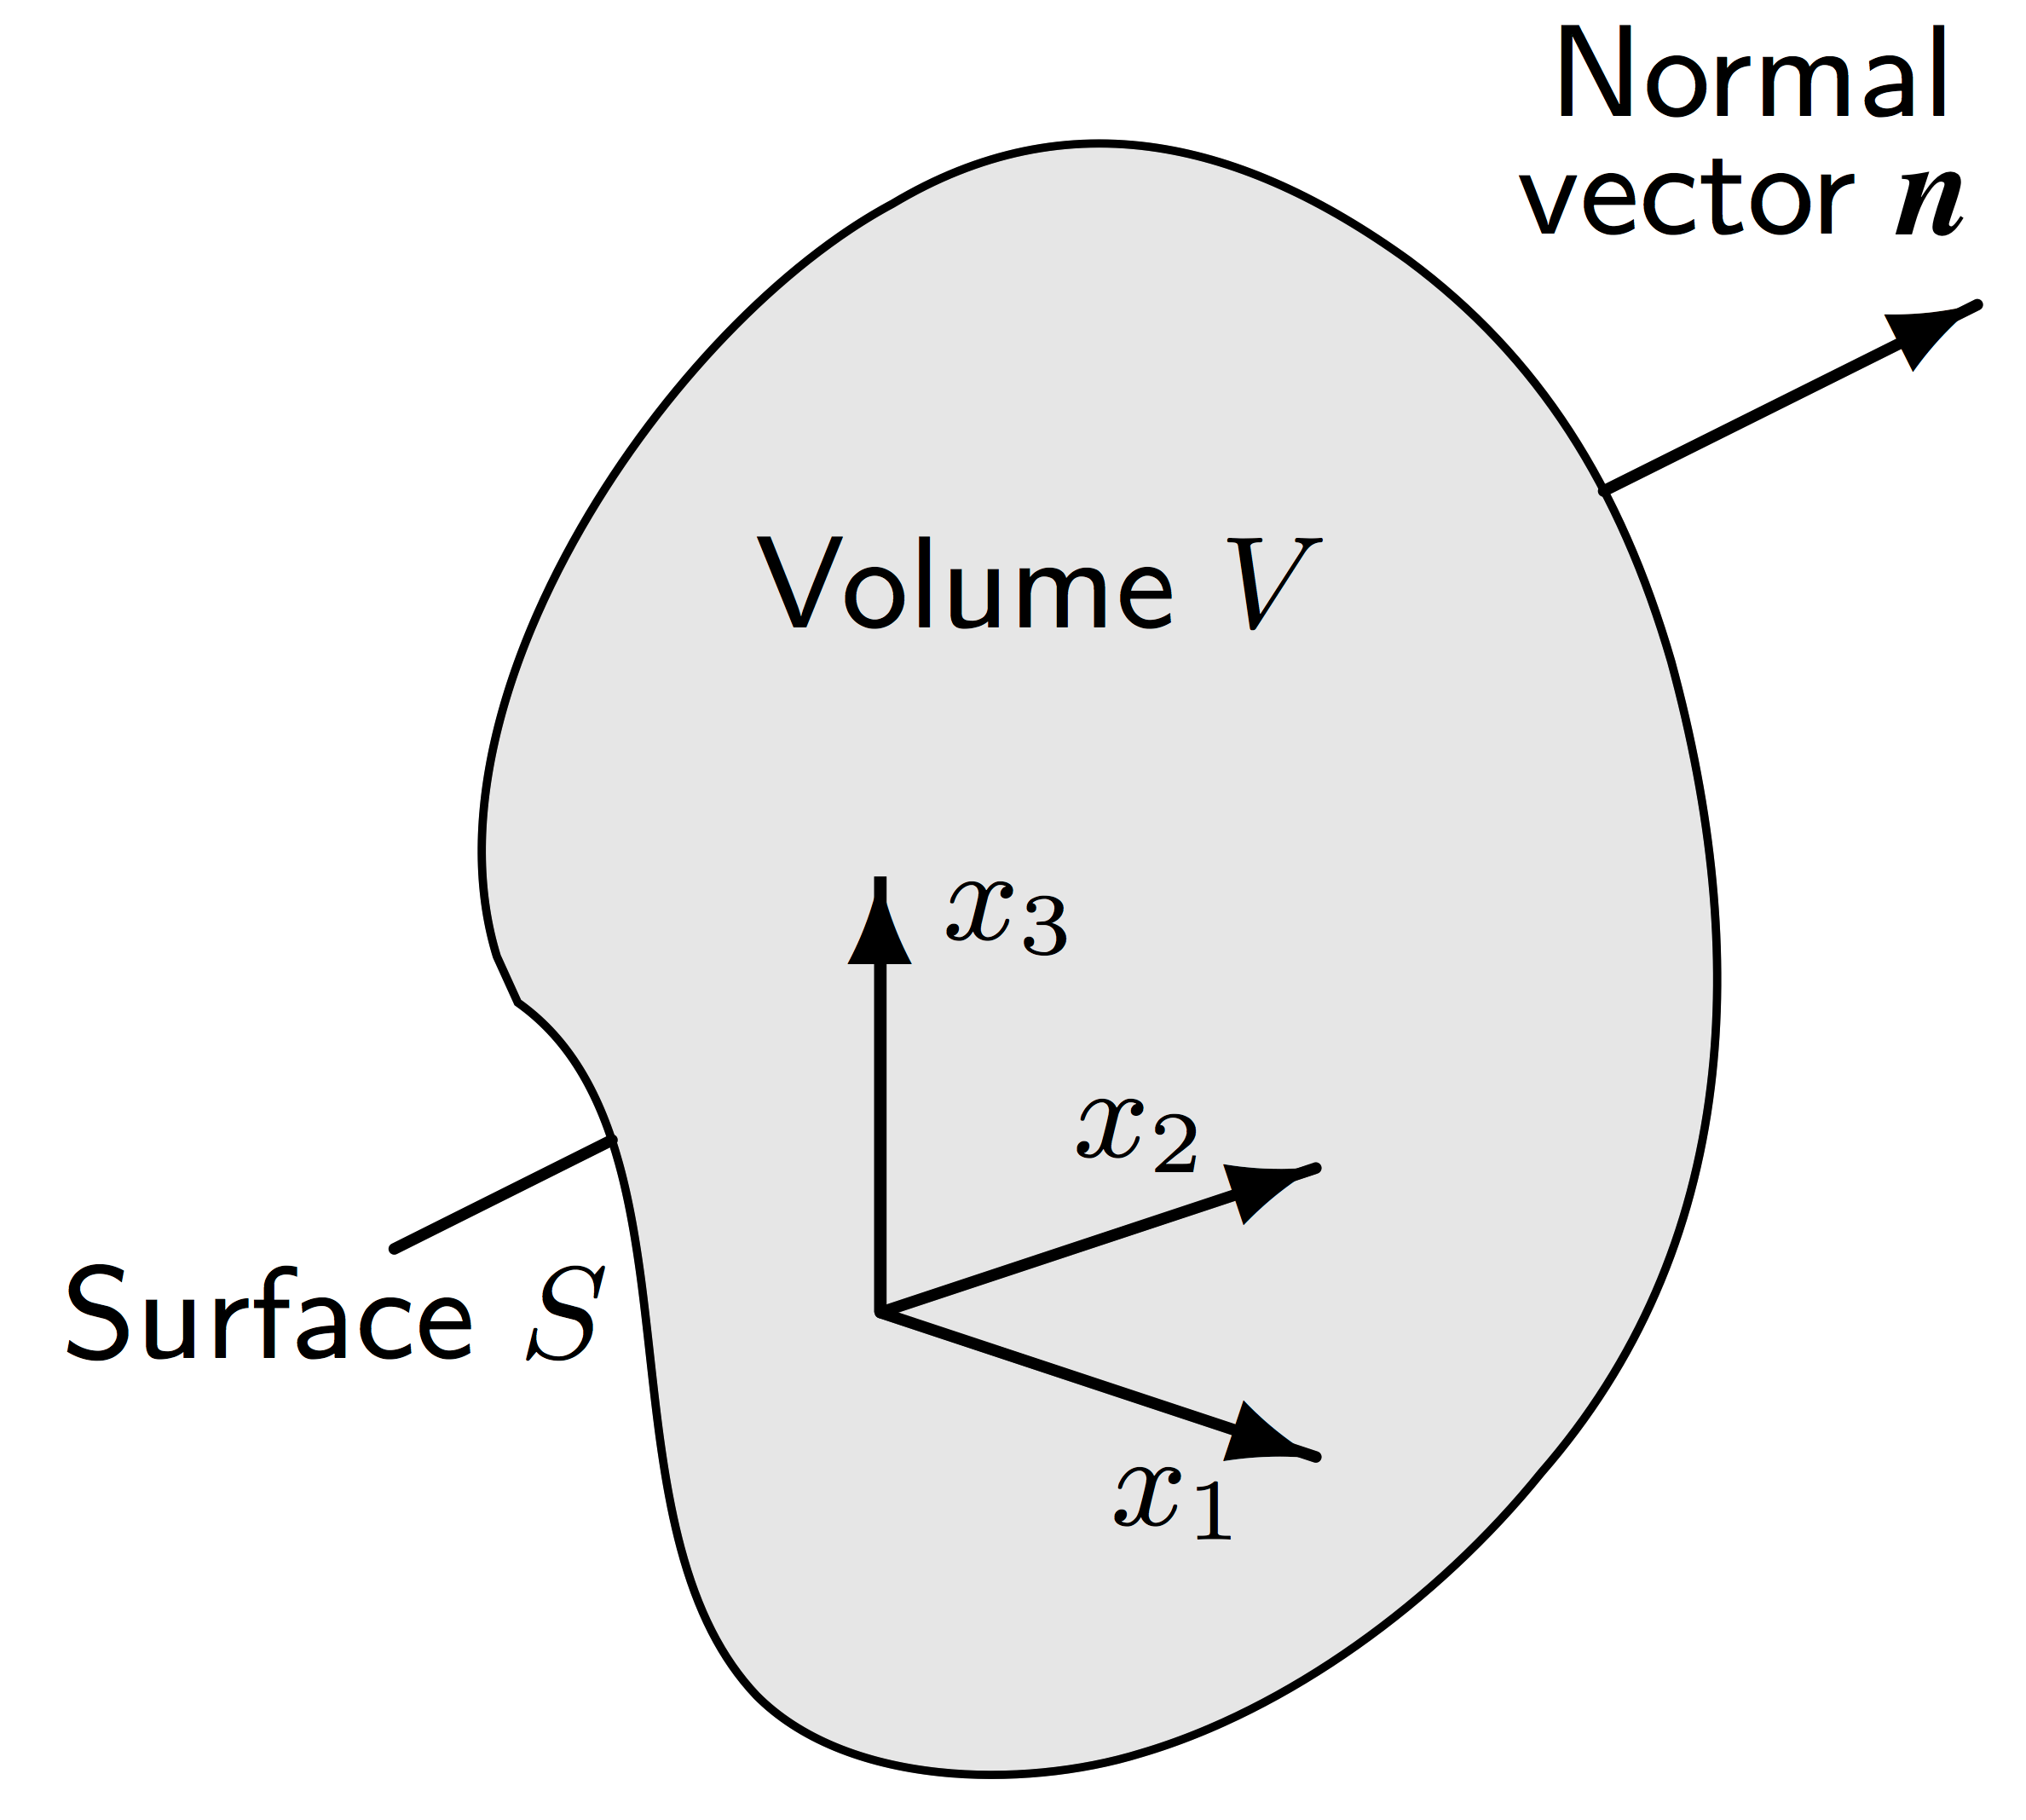
\includegraphics[width=0.4\textwidth]{chap1/include/figures/control_volume.png}
\caption[Control volume for the finite volume method.]{Control volume for the finite volume method (adapted from M. Sch\"afer, Computational engineering: Introduction to numerical methods, Springer, Berlin, 2006).}
\label{chap1:fig:computational_methods_control_volume}
\end{figure}

In practice, the finite volume method consists in applying the same procedure considering the cells of the mesh as the control volumes.
For instance, consider a structured mesh with some inner cell denoted as $c$ and faces denoted as $n$, $e$, $s$, and $w$, as illustrated in Figure~\ref{chap1:fig:computational_methods_finite_volume_method_orthogonal}.
The volume of the cell is denoted as $\left\vert c\right\vert$, whereas the areas of the faces are denoted as $\left\vert n\right\vert$, $\left\vert e\right\vert$, $\left\vert s\right\vert$, and $\left\vert w\right\vert$.
The mid-point of the cell is denoted as $P$, the mid-points of the neighbour cells are noted as $N$, $E$, $S$, and $W$, and the outward unit normal vectors denoted as $\bm{n}_{\textrm{N}}$, $\bm{n}_{\textrm{E}}$, $\bm{n}_{\textrm{S}}$, and $\bm{n}_{\textrm{W}}$.
The unknown temperature is represented piece-wisely at the mid-points of the cells, where for the previous points are denoted as $T_{\textrm{P}}$, $T_{\textrm{N}}$, $T_{\textrm{E}}$, $T_{\textrm{S}}$, and $T_{\textrm{W}}$, which are unknowns of the discrete problem.

\begin{figure}[!htp]
\centering
\begin{tabular}{@{}c@{\hskip 1.5cm}c@{}}
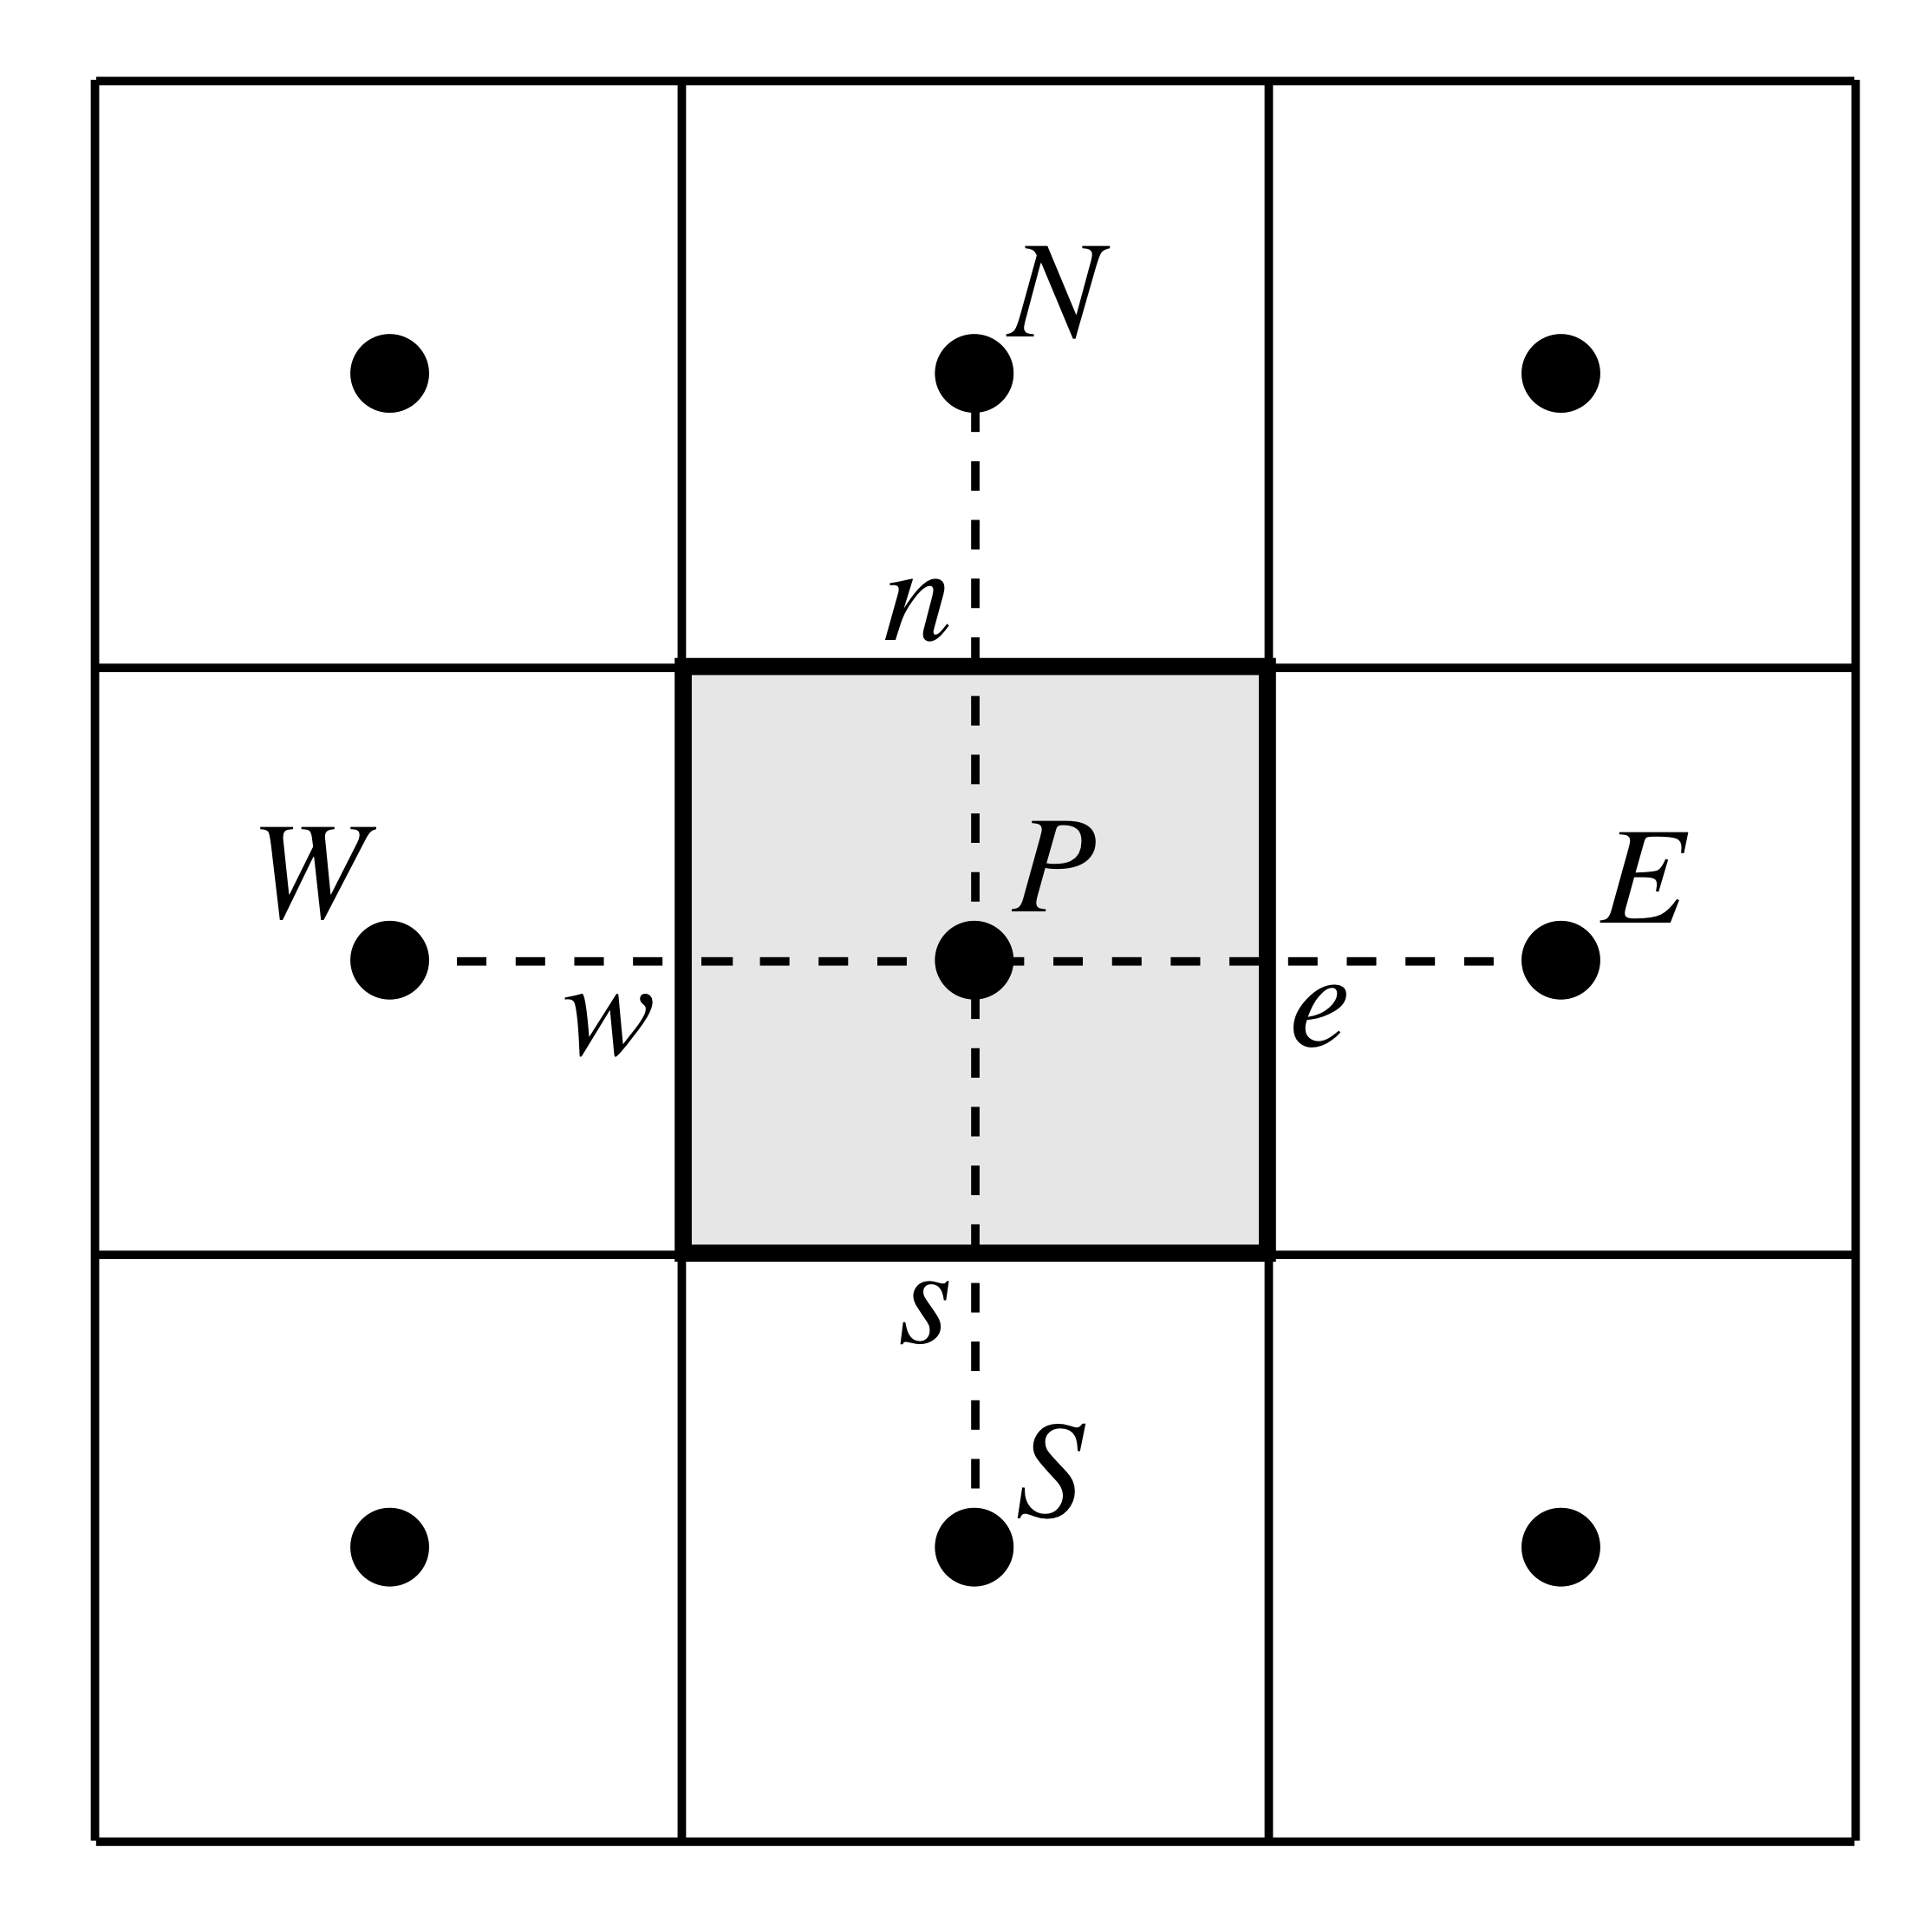
\includegraphics[width=0.4\textwidth]{chap1/include/figures/finite_volume_method_inner.png}
& 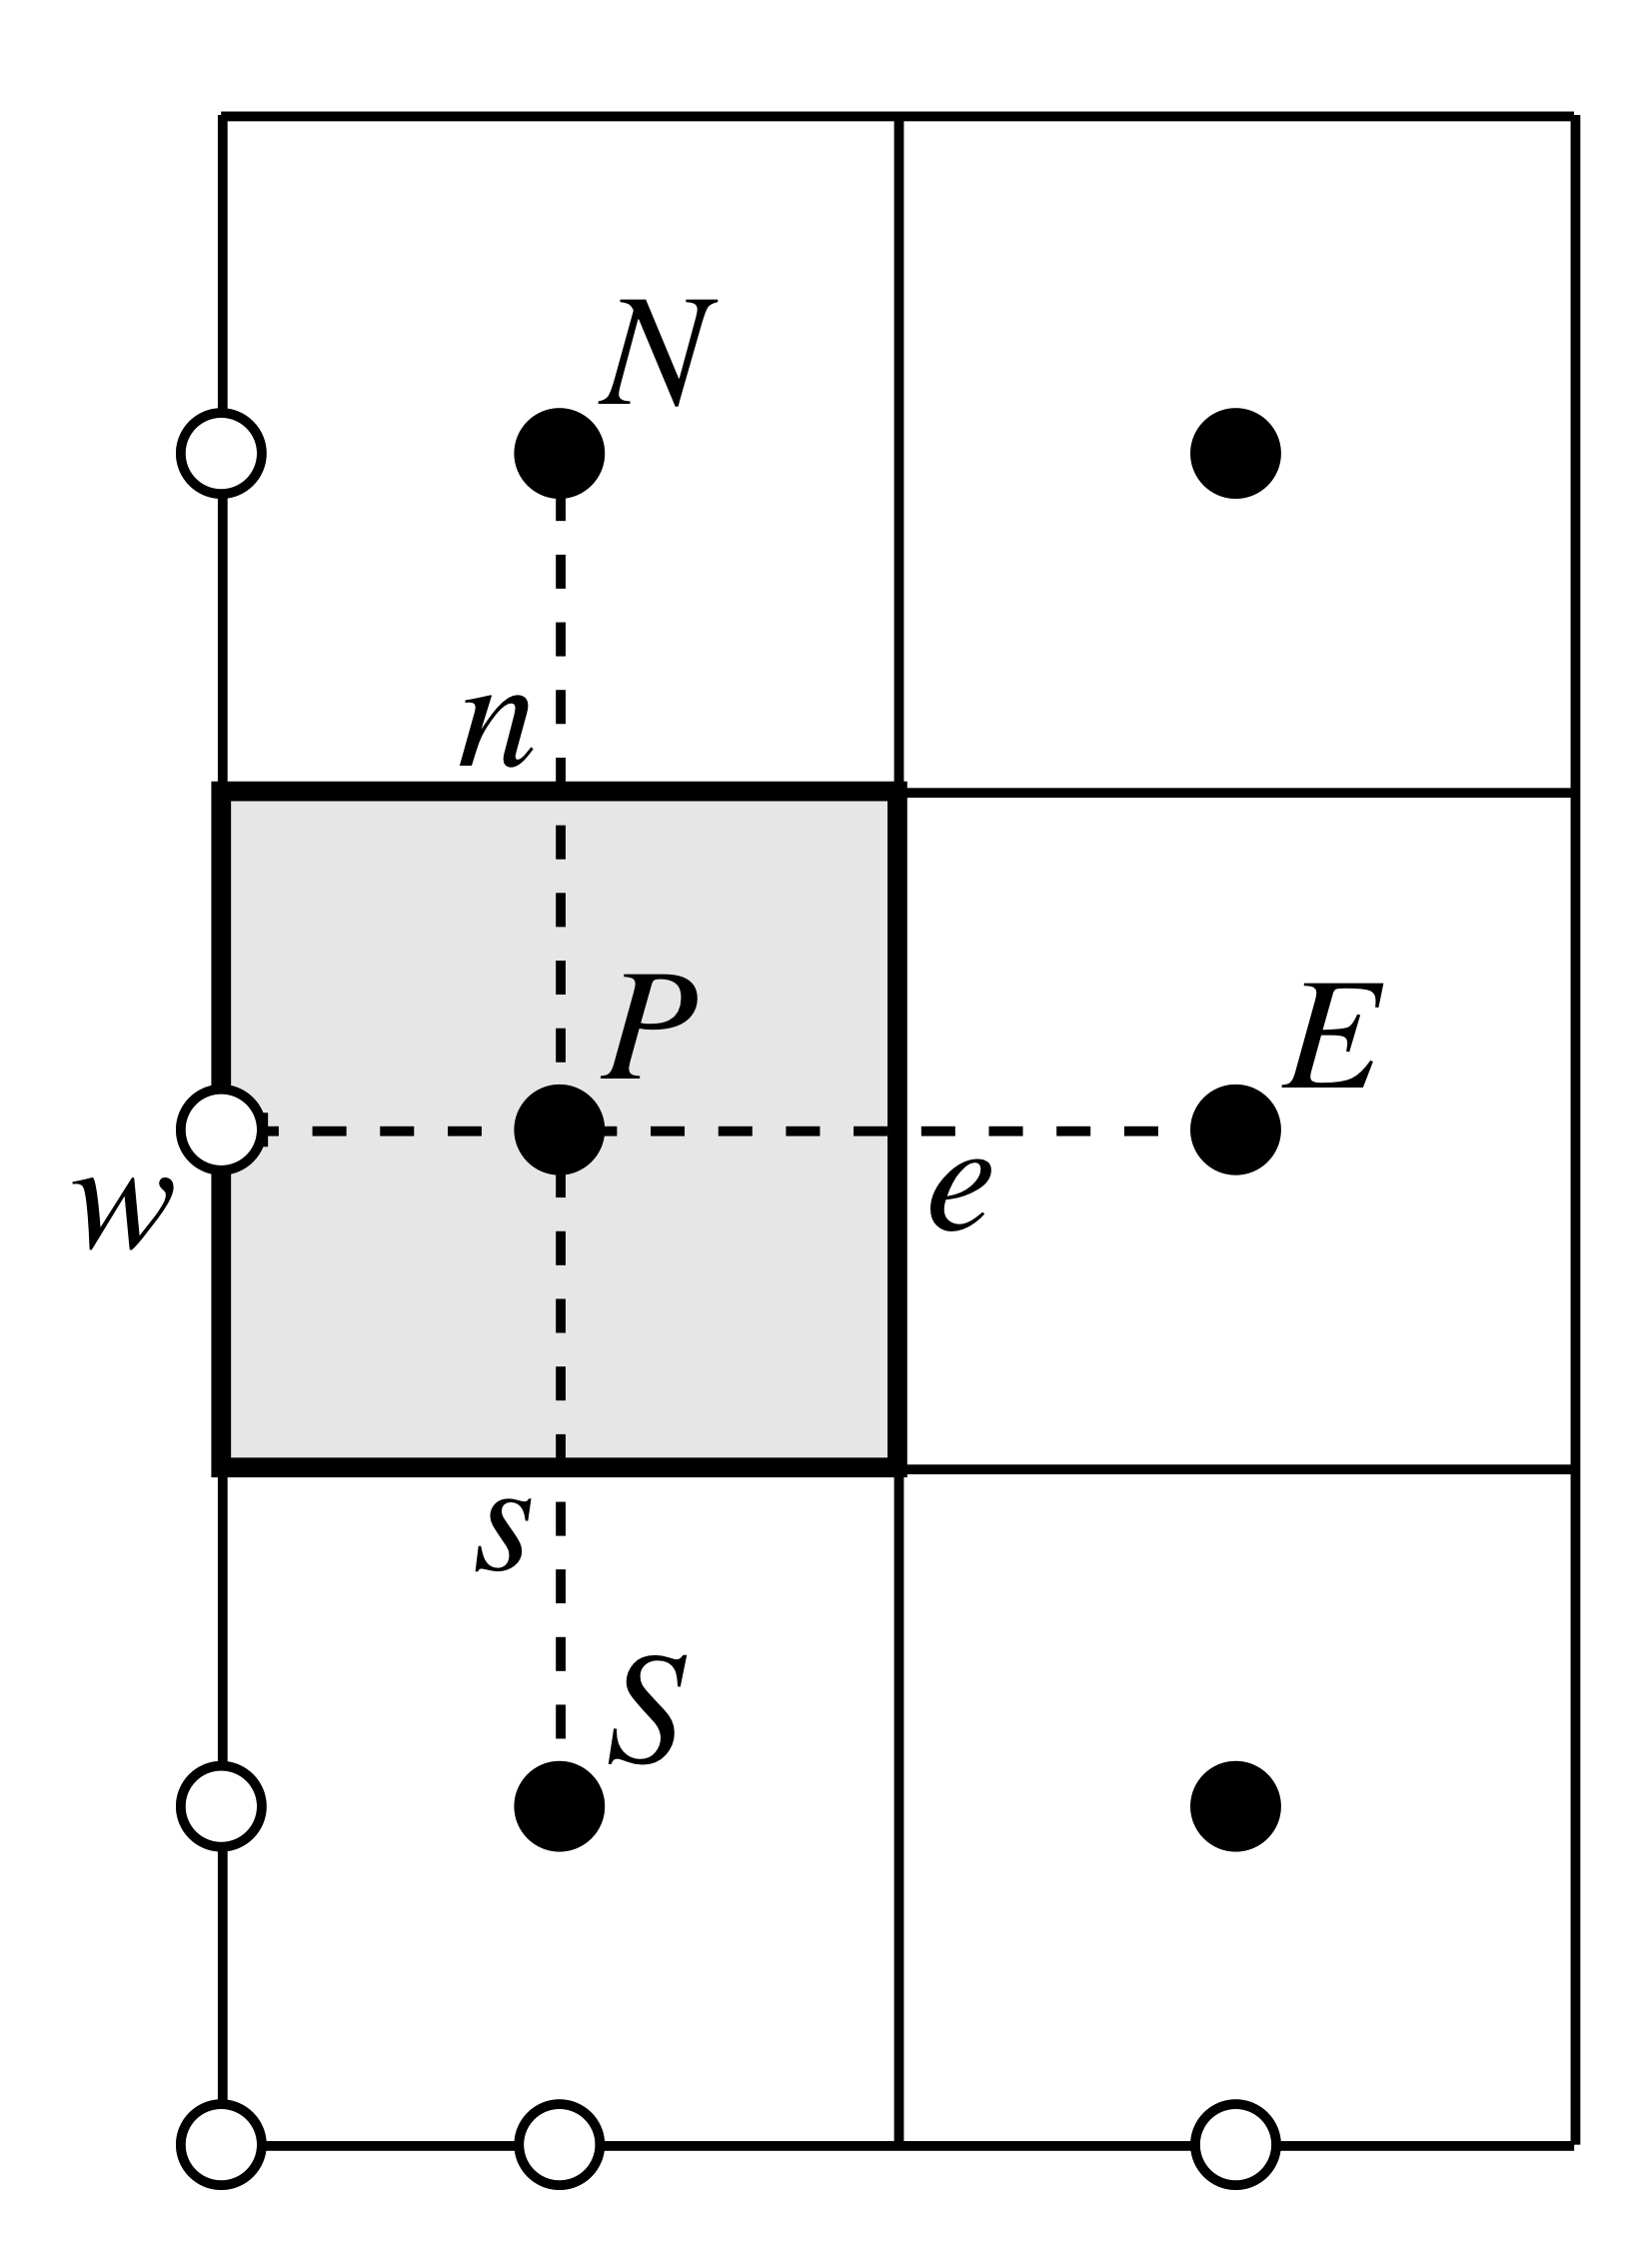
\includegraphics[width=0.3\textwidth]{chap1/include/figures/finite_volume_method_boundary.png}\\
\small (a) Inner cell. & \small (b) Boundary cell.
\end{tabular}
\caption[Notations for the finite volume method with a structured orthogonal mesh.]{Notations for the finite volume method in a structured orthogonal mesh (adapted from M. Sch\"afer, Computational engineering: Introduction to numerical methods, Springer, Berlin, 2006).}
\label{chap1:fig:computational_methods_finite_volume_method_orthogonal}
\end{figure}

The division of the surface integral of Equation~\cref{chap1:eq:computational_methods_heat_conduction3} into the different cell faces, gives
\begin{equation}
\int_{n}-\kappa\nabla T\cdot\bm{n}_{\textrm{N}}\textrm{d}\bm{x}+\int_{e}-\kappa\nabla T\cdot\bm{n}_{\textrm{E}}\textrm{d}\bm{x}+\int_{s}-\kappa\nabla T\cdot\bm{n}_{\textrm{S}}\textrm{d}\bm{x}+\int_{w}-\kappa\nabla T\cdot\bm{n}_{\textrm{W}}\textrm{d}\bm{x}=\int_{c}f\textrm{d}\bm{x}.
\label{chap1:eq:computational_methods_heat_conduction4}
\end{equation}
Equation~\cref{chap1:eq:computational_methods_heat_conduction4} constitutes a generic formulation of the finite volume method, where no approximation were introduced until this point.
However, the surface integrals of the normal temperature derivative on the faces and the volume integral of the source term in the cell have to be discretized to built the equivalent system of linear algebraic equations.
In that regard, there is an uncountable number of numerical schemes that emerged within the finite volume method, having in common Equation~\cref{chap1:eq:computational_methods_heat_conduction4} for the problem discretization.
A simple and straightforward numerical approximation of the surface integrals in Equation~\cref{chap1:eq:computational_methods_heat_conduction4} is given as
\begin{align}
&\int_{n}-\kappa\nabla T\cdot\bm{n}_{\textrm{PN}}\textrm{d}\bm{x}\approx -\kappa\frac{T_{\textrm{N}}-T_{\textrm{P}}}{\left\vert N_{y}-P_{y}\right\vert}\left\vert n\right\vert,\\
&\int_{e}-\kappa\nabla T\cdot\bm{n}_{\textrm{PE}}\textrm{d}\bm{x}\approx -\kappa\frac{T_{\textrm{E}}-T_{\textrm{P}}}{\left\vert E_{x}-P_{x}\right\vert}\left\vert e\right\vert,\\
&\int_{s}-\kappa\nabla T\cdot\bm{n}_{\textrm{PS}}\textrm{d}\bm{x}\approx -\kappa\frac{T_{\textrm{S}}-T_{\textrm{P}}}{\left\vert S_{y}-P_{y}\right\vert}\left\vert s\right\vert,\\
&\int_{w}-\kappa\nabla T\cdot\bm{n}_{\textrm{PW}}\textrm{d}\bm{x}\approx -\kappa\frac{T_{\textrm{W}}-T_{\textrm{P}}}{\left\vert W_{x}-P_{x}\right\vert}\left\vert w\right\vert,
\end{align}
which is equivalent to a finite difference approximating the normal derivative of the temperature based on the associated discrete variables.
In the case of a cell with a boundary face, as illustrated in Figure~\ref{chap1:fig:computational_methods_finite_volume_method_orthogonal}, a different approximation is provided considering the boundary condition prescribed on the associated boundary of the domain.
Moreover, in the case of structured or unstructured non-orthogonal meshes, as illustrated in Figure~\ref{chap1:fig:computational_methods_finite_volume_method_nonorthogonal}, such a simple scheme requires non-orthogonal corrections to preserve the consistency of the surface integral approximations.
A usual strategy consists in fixing the finite difference between the cell mid-points with a correction based on the vertex points, for which accurate and robust numerical techniques for interpolation of the solution at the vertices are available~\cite{chap1:2014costa}.
On the other side, the volume integral of the source terms is straightforwardly approximated with the value of the given function at the cell mid-point, denoted as $f_{\textrm{P}}$.

\begin{figure}[!htp]
\centering
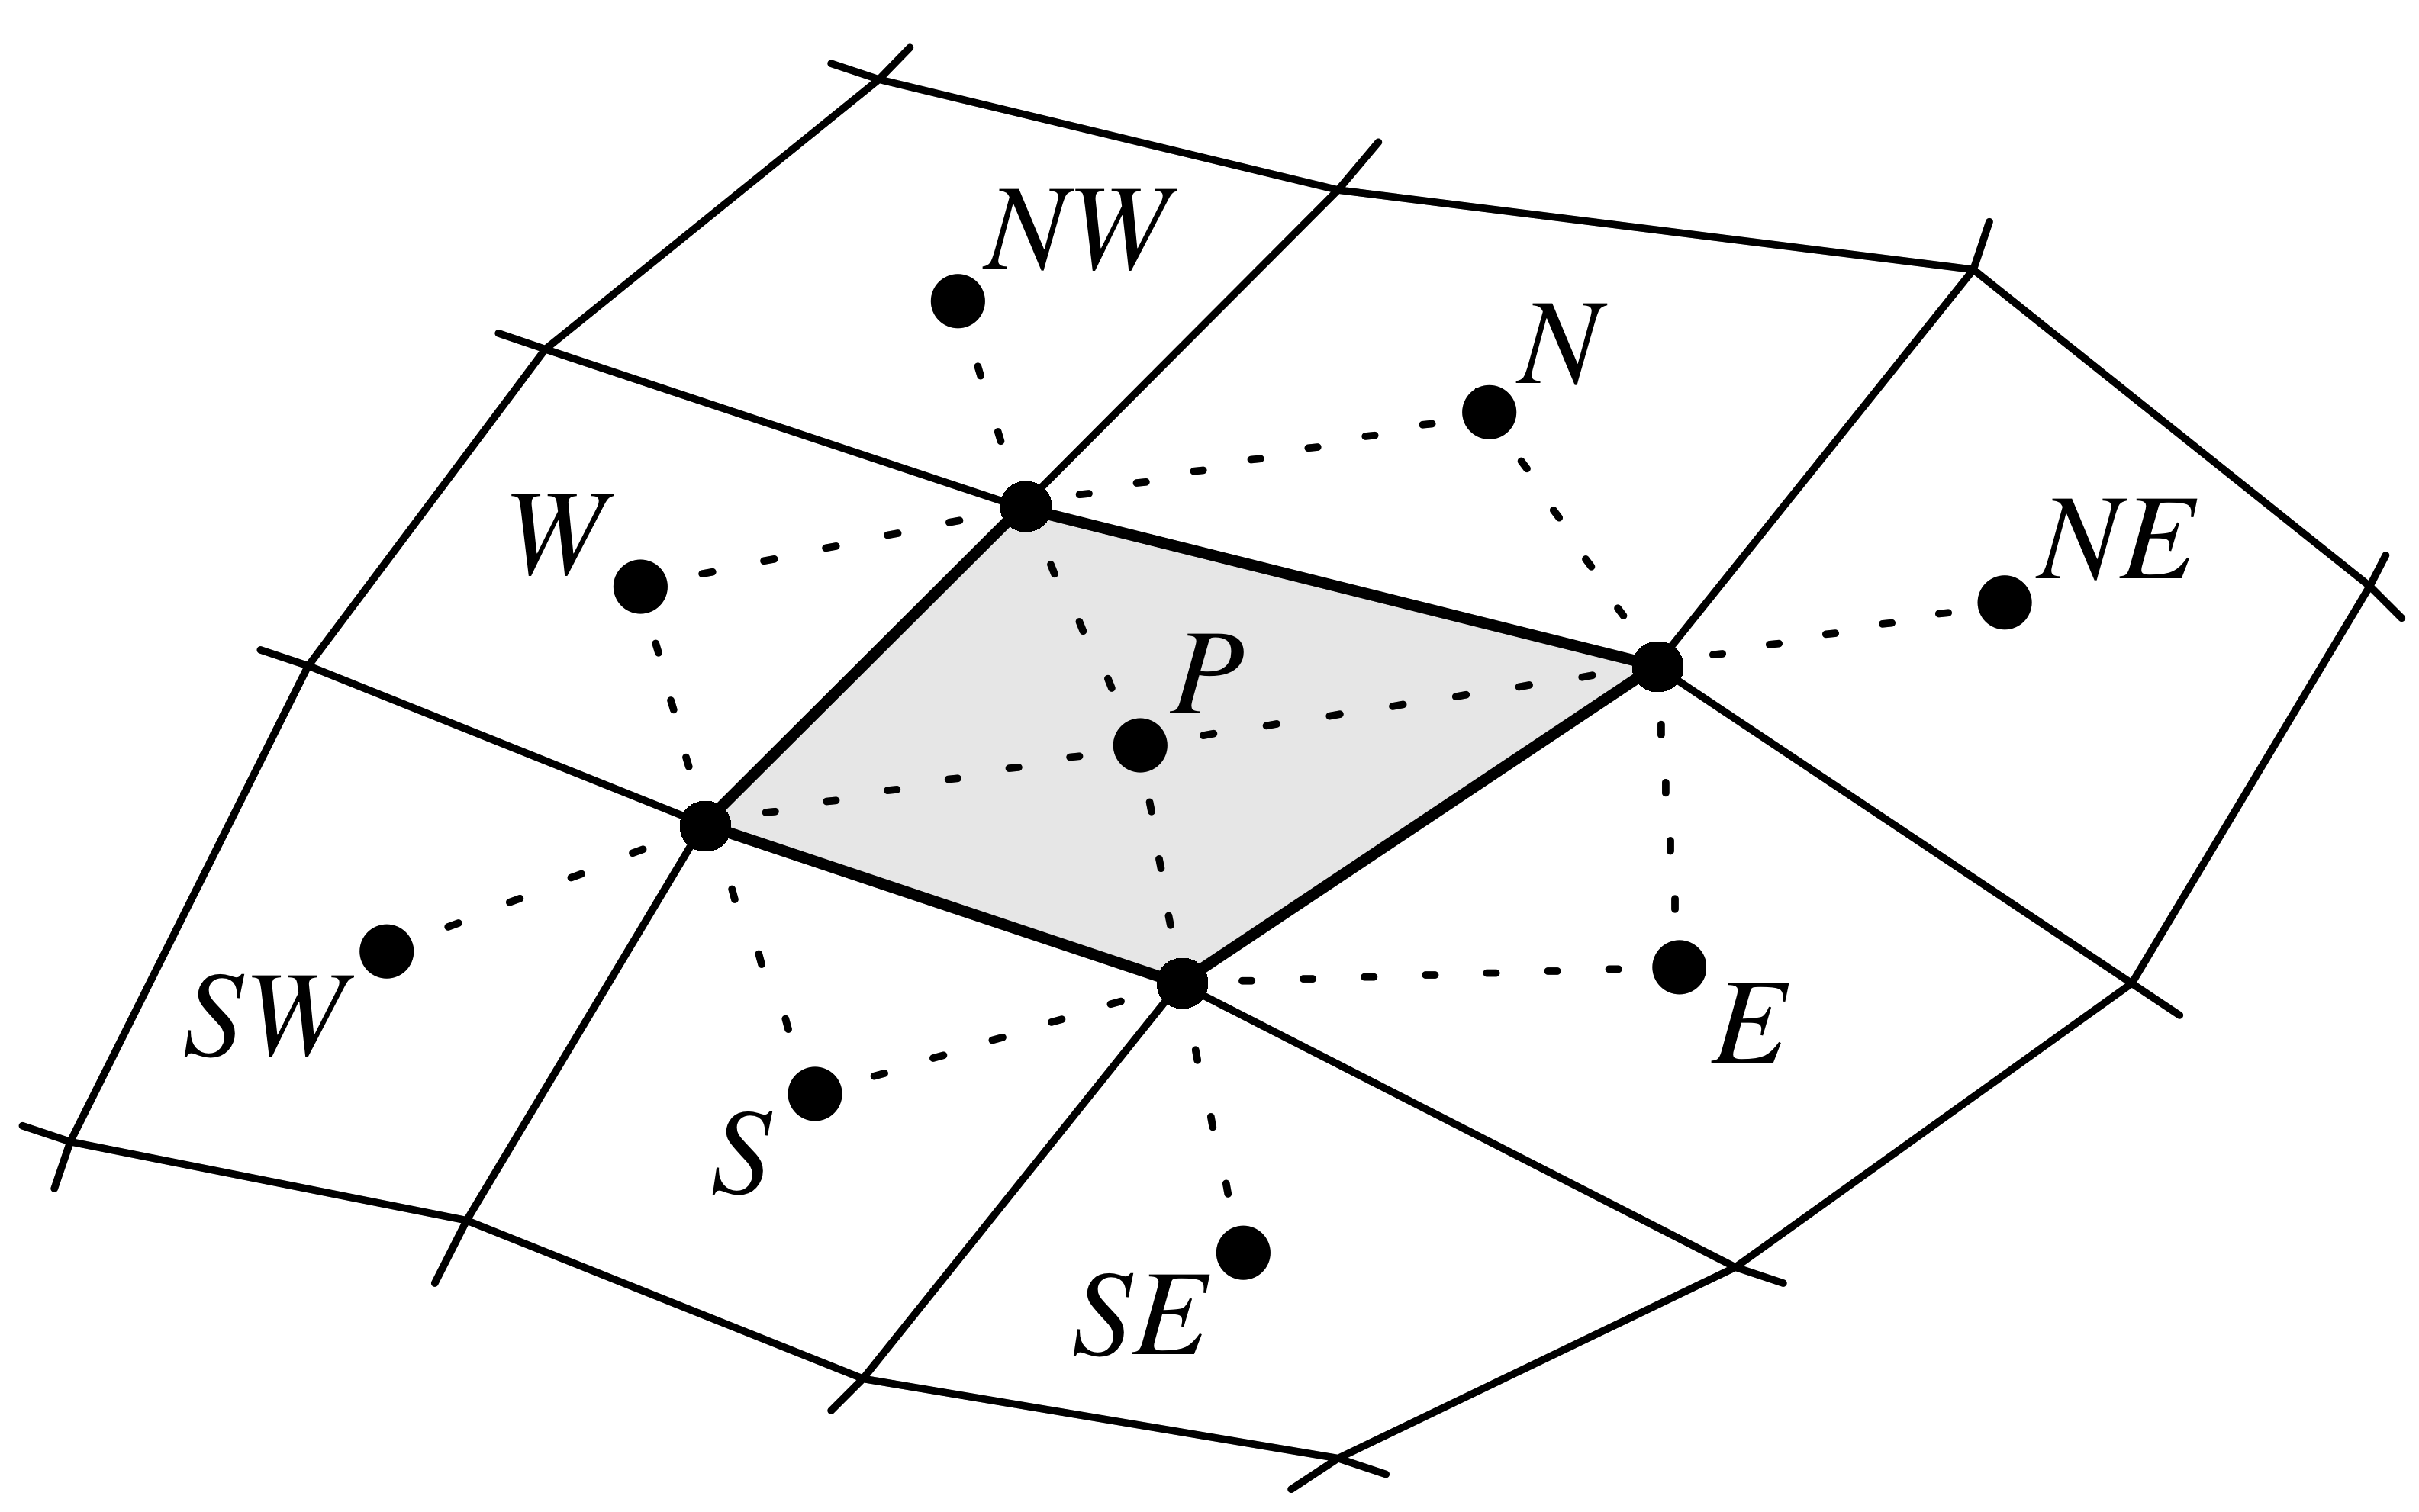
\includegraphics[width=0.5\textwidth]{chap1/include/figures/finite_volume_method_nonorthogonal.png}
\caption[Mesh notations for the finite volume method with a non-orthogonal mesh.]{Mesh notations for the finite volume method with a structured non-orthogonal mesh (adapted from M. Sch\"afer, Computational engineering: Introduction to numerical methods, Springer, Berlin, 2006).}
\label{chap1:fig:computational_methods_finite_volume_method_nonorthogonal}
\end{figure}

Finally, the discrete problem consists in rewritten Equation~\cref{chap1:eq:computational_methods_heat_conduction4} with the numerical approximations of the surface and volume integrals, given as
\begin{equation}
-\kappa\frac{T_{\textrm{N}}-T_{\textrm{P}}}{\left\vert N_{y}-P{y}\right\vert}\left\vert n\right\vert-\kappa\frac{T_{\textrm{E}}-T_{\textrm{P}}}{\left\vert E_{x}-P_{x}\right\vert}\left\vert e\right\vert-\kappa\frac{T_{\textrm{S}}-T_{\textrm{P}}}{\left\vert S_{y}-P_{y}\right\vert}\left\vert s\right\vert-\kappa\frac{T_{\textrm{W}}-T_{\textrm{P}}}{\left\vert W_{x}-P_{x}\right\vert}\left\vert w\right\vert=f_{\textrm{P}}\left\vert c\right\vert,
\label{chap1:eq:computational_methods_heat_conduction5}
\end{equation}
which translates into a linear algebraic relation between the discrete variables of the temperature at the cell mid-points.
The discretization procedure is repeated for each cell of the mesh, which provides the same number of linear algebraic equations as the number of discrete variables.
A system of linear equations is then assembled from these algebraic equations, which is solved using matrix algebra techniques.

In the previous example, the finite volume method has a straightforward physical interpretation since the surface integrals on the control volume surface correspond to the conductive heat flux.
Indeed, this translates into the First Law of thermodynamics where the quantity of heat supplied to the control volume has to be equal to the quantity of heat leaving the control volume plus or minus the heat sources or sinks.
For other governing equations, by providing the conservation of some quantity in the integral form, the finite volume method leads to the same conservation principle in terms of fluxes of some physical quantity.
Indeed, the conservation of specific physical quantities, such as energy and mass, is only mathematically translated when associated partial differential equations are written in the integral form over some control volume.
This conservation principle is not only satisfied at the level of the continuous problem but also at the level of the discrete problem based on the balance of the fluxes in the cell.
Moreover, the conservation principle in the discrete form is also satisfied regardless of the number or size of cells in the mesh.
On the other side, the conservation principle, which is intrinsically satisfied in the finite volume method, is not, however, necessarily verified in the context of the finite difference method or the finite element methods.
Another advantage of the finite volume method is the capability to handle any type of mesh, which becomes of interest to work with complex geometries, as often occurs in polymer processing applications.
Additionally, the lower abstraction level and higher physical meaning, makes the finite volume method easier to understand and implement, and, thus, more appealing for engineers than the finite element method.

The accuracy of the discretization method depends upon the governing equation, problem geometry, mesh generation, and flux approximation on the control volume surface.
Significant developments took place after the work of Patankar for structured meshes and comprehensive literature exists with several classes of methods in the context of the finite volume method, summarized to the following.
The classical two-points flux finite volume method~\cite{chap1:1991caia,chap1:1991caib,chap1:2000eymard,chap1:2001eymard}, also referred to as the FV$4$ method, extends the original Patankar method to unstructured meshes, but an orthogonality condition is required to allow admissible diffusive fluxes.
The diamond-cell finite volume method~\cite{chap1:1999coudierea,chap1:1999coudiereb,chap1:2008manzini}, was introduced for unstructured non-orthogonal meshes (no orthogonality condition required) and is based on local linear reconstructions to compute the gradients on each control volume face.
The drawback of the diamond-cell finite volume method is the lack of symmetry and the difficult and limited numerical analysis.
The discrete duality finite volume method~\cite{chap1:2000hermeline,chap1:2005domelevo,chap1:2010coudiere}, also referred to as the DDFV method, handles unstructured non-orthogonal and possibly non-conformal meshes and satisfies the div-grad duality intrinsically at the discrete level.
Contrarily to the previous methods, the DDFV finite volume method requires unknowns at the vertices of the mesh as well as dual and diamond control volumes in addition to the primal ones.
On the other side, the DDFV method is symmetric and numerical analysis is straightforward and general.
More recently, to design efficient discretization schemes, several finite volume methods have been proposed, such as the mixed-hybrid methods~\cite{chap1:2006droniou,chap1:2008eymard} or the mimetic methods~\cite{chap1:2005brezzi,chap1:2008cangiani}, among others.

In the case of fluid flow problem, specific numerical techniques are required to correctly solve the div-grad duality between velocity and pressure arising from the balance of momentum and continuity equations~\cite{chap1:1967chorin,chap1:1996ferziger,chap1:1983pironneau,chap1:1984crochet,chap1:1985peyret,chap1:1987temam,chap1:2014zienkiewicz}.
In that regard, discretization methods are also classified as staggered, when the discrete variables for the velocity and pressure are defined in different meshes (primal and diamond meshes)~\cite{chap1:2004piller,chap1:2004vidovic,chap1:2006kampanis}, or as collocated, when both discrete variables are defined in the same mesh~\cite{chap1:1998oliveira,chap1:2009eymard,chap1:2014shang}.
Moreover, the discretization methods are also classified as coupled when the governing equations are discretized and solved in the same system of linear equations, leading to a saddle point problem, or as segregated when a projection method in the divergence-free space is used, such as the classical SIMPLE, SIMPLEC, SIMPLER, and PISO methods~\cite{chap1:2001brown,chap1:2006guermont,chap1:2009gao,chap1:2009griffith}.

\subsection{Very high-order of convergence}
\label{chap1:subsec:computational_methods_high_order_of_convergence}

The convergence order of the discretization method measures the rate at which the approximate solution error decreases under mesh refinement, that is, the same as increasing the number of unknowns.
Classical discretization methods provide a second-order of convergence, whereas achieving higher-orders of convergence usually requires more complex numerical techniques and more laborious implementations.
Very high-order accurate methods are herein defined as those having more than the second-order of convergence for the obtained approximate solution error.
Such class of methods have historically emerged to capture, with higher accuracy and resolution than the classical ones, shocks and discontinuities in fluid flow hyperbolic-dominated problems, such as the Euler equation for compressible inviscid fluid flows or the shallow water equations.
In that context, discretization methods with third and fourth-orders of convergence have been a standard in aeronautic and nuclear research to solve engineering problems with non-smooth solutions.
Unfortunately, the computational modelling software commonly used in the polymer processing industry still relies on classical discretization methods with a first- or second-order of convergence.

The most prominent benefit of very high-order accurate methods is to obtain a higher accuracy for the same mesh than low-order accurate methods, such as first- or second-orders, as illustrated in Figure~\ref{chap1:fig:computational_methods_convergence_order}.
Since the approximate solution error decreases faster when employing very high-order accurate methods, this benefit is more pronounced as the accuracy requirements for the application increases.
In theory, low-order accurate methods are still capable of achieving the same levels of accuracy increasing the mesh refinement, but with a much higher computational cost and limited in practice by the memory capabilities of computers.
Consequently, the memory requirements for demanding applications may exceed the available computer memory, for which very high-order accurate methods are also a promising workaround.
From the computational efficiency viewpoint, very high-order accurate methods provide higher accuracy but, as a consequence of their increased complexity, also require more execution time per iteration for the same mesh than low-order accurate methods.
In that regard, there is a non-trivial trade-off between accuracy and execution time, which is usually in favour of very high-order accurate methods, as illustrated in Figure~\ref{chap1:fig:computational_methods_convergence_order}.
That is, increasing the convergence order to achieve a certain level of accuracy is usually preferable than refining the mesh with low-order accurate methods, which typically lead to a higher execution time besides the inevitable memory limitations.
Notice that time discretization of unsteady problems with very high-order of convergence is also possible, although the literature is more scarce than for the spatial discretization.
Nevertheless, these methods are also capable of providing more accurate approximate solutions for long-time simulations, when compared with low-order accurate methods.

\begin{figure}[!htb]
\centering
\begin{tabular}{@{}c@{}c@{}}
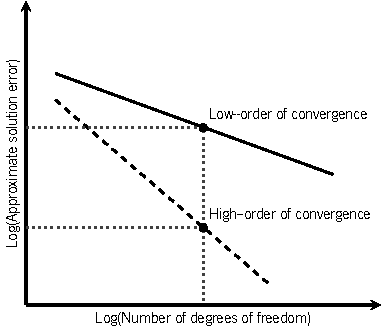
\includegraphics[width=0.5\textwidth]{chap1/include/tikz/error_vs_dof.pdf}
& 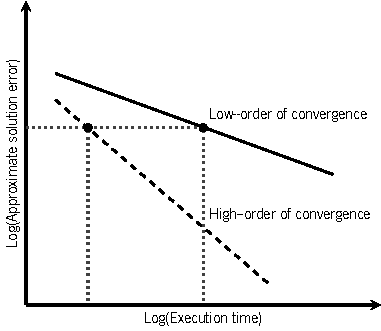
\includegraphics[width=0.5\textwidth]{chap1/include/tikz/error_vs_time.pdf}\\
\small (a) Number of degrees of freedom. & \small (b) Execution time.
\end{tabular}
\caption{Typical convergence curves for low- and very high-orders accurate methods.}
\label{chap1:fig:computational_methods_convergence_order}
\end{figure}

In fluid flow hyperbolic-dominated problems, the essentially non-oscillatory method, or its weighted variant, has been widely used to achieve the third- and fifth-orders of convergence~\cite{chap1:1997ollivier,chap1:2002hernandez,chap1:2002ollivier,chap1:2009toro,chap1:2011ivan,chap1:2018barth}.
The method avoids that spurious oscillations are captured due to the Gibbs phenomenon~\cite{chap1:1997gottlieb}, whereas other approaches have been recently developed, as the multi-dimensional optimal order detection method~\cite{chap1:2011clain,chap1:2012diot,chap1:2013diot}.
On the other side, elliptic-dominated problems, as those concerning the heat transfer in polymer processing applications, have not received the same attention within the development of very high-order accurate methods.

% end of file
